\chapter{Probabilistic Language Model}
\section{Introduction}
Language model is used to estimate the probability of the word sequences and to estimate the probability of a word following the sequence of words. The concept can be used to auto-complete a sentence with most likely suggestions as shown below:
\begin{figure}[h]
	\centering
	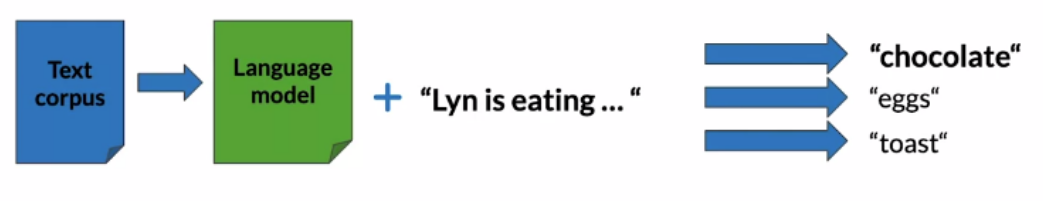
\includegraphics[scale = 0.35]{autoComplete.png}
	\caption{Language Model for Auto-complete}
	\label{fig:my_label}
\end{figure}

\noindent
Some other applications of the language model are:
\begin{enumerate}
	\item Speech Recognition
	\item Spelling Correction
	\item Augmentative Communication
\end{enumerate}

\section{N-gram}
A N-gram is a sequence of N-words. For example:

\textbf{Corpus :} I am happy because I am learning.

\textbf{Uni-grams :} \{I, am, happy, because, I, am, learning \}

\textbf{Bi-grams :} \{I am, am happy, happy because, …\}

\textbf{Tri-grams :} \{I am happy, am happy because, …\}

\section{Sequence Notation}
Let's define a standard sequence notation to represent the sequence of words in our corpus.	Let our corpus be as shown below where n$^{th}$ is represented as W$_n$.
Let the number of words in the corpus be m = 500

\textbf{Corpus:} This is great. ... teacher drinks tea.

Hence,  W$_1$ = This, W$_2$ = is, W$_3$ = great and so on...

Let us represent the sequence of words as W$_s^e$ where s represent the starting index and e represent the ending index of the words in the corpus. So,

W$_1^m$ = W$_1$ W$_2$ W$_3$ ....................  W$_{m-1}$ W$_m$

Similarly,  W$_1^3$ = W$_1$ W$_2$ W$_3$ = This is great

\section{N-gram Probability}
N-gram probability is the probability of the occurrence of the sequence of N-words in a corpus. From uni-gram, bi-gram  and tri-gram probability, we can deduce for N-gram probability denoted by $P(W_N | W_1^{N-1})$ as

\begin{equation}
	P(W_N | W_1^{N-1}) = \frac{C(W_1^{N - 1} \, W_N)}{C(W_1^{N - 1})} = \frac{C(W_1^N)}{C(W_1^{N - 1})}
\end{equation}

\subsection{Uni-gram Probability}
Uni-gram Probability is the probability of occurrence of a word in a given corpus.

\textbf{Corpus :} I am happy because I am learning.

\textbf{Size of corpus : } m = 7
\begin{equation}
	P(I) = \frac{2}{7}
\end{equation}
\begin{equation}
	P(happy) = \frac{1}{7}
\end{equation}

Hence, we can see that Probability of uni-gram is given by:
\begin{equation}
	P(w) = \frac{C(w)}{m}
\end{equation}
where C(w) = frequency of the word in the corpus

\subsection{Bi-gram Probability}
Bi-gram Probability is the probability of occurrence of sequence of two words in a corpus.
\\
\textbf{Corpus :} I am happy because I am learning.
\\
\textbf{Size of corpus : } m = 7
\begin{equation}
	P(am | I) = \frac{C(I\, am)}{C(I)} = \frac{2}{2} = 1
\end{equation}
\begin{equation}
	P(happy | I) = \frac{C(I \, happy)}{C(I)}= \frac{0}{7} = 0
\end{equation}
\begin{equation}
	P(learning | am) = \frac{C(am \, learning)}{C(am)} = 1 / 2
\end{equation}

Hence, we can see that Probability of bi-gram is given by:
\begin{equation}
	P(y | x) = \frac{C(x\, y)}{C(x)}
\end{equation}
where C(w) = frequency of the word in the corpus

\subsection{Tri-gram Probability}
Tri-gram Probability is the probability of the occurrence of the sequence of three words in a corpus.
\\
\textbf{Corpus :} I am happy because I am learning.
\\
\textbf{Size of corpus : } m = 7
\begin{equation}
	P(happy | I\, am) = \frac{C(I\, am \, happy)}{C(I \, am)} = \frac{1}{2}
\end{equation}

Hence, we can see that Probability of bi-gram is given by:
\begin{equation}
	P(W_3 | W_1^2) = \frac{C(W_1^2\, W_3)}{C(W_1^2)} = \frac{C(W_1^3)}{C(W_1^2)}
\end{equation}
where C(w) = frequency of the word in the corpus



\section{Probability of a sequence}
From the conditional probability and chain rule, we have
\begin{equation}\label{CP}
	P(B|A) = \frac{P(A, B)}{P(A)}
\end{equation}

From (\ref{CP}), we get
\begin{equation}\label{CP1}
	P(A, B) = P(A) . P(B | A)
\end{equation}

Using (\ref{CP1}), we can deduce
\begin{equation}
	P(A, B, C, D) = P(A).P(B|A).P(C|A, B).P(D|A, B, C)
\end{equation}

Now, the probability of the sequence of words: "the teacher drinks tea" is given by:

\begin{flalign}
	\begin{aligned}
		 & P(the\, teacher\, drinks\, tea) = P(the) . P(teacher | the) \\
		 & P(drinks | the\, teacher) . P(tea | the\, teacher\, drinks)
	\end{aligned}
\end{flalign}

\section{Approximation of Sequence Probability}
When using n-gram language model, the exact sentence for the required n-gram might not be present exactly in corpus due to which the frequency of the words sequence becomes zero and hence the probability. For example:

\textbf{Input :} the teacher drinks tea

P(the\, teacher\, drinks\, tea) = P(the) . P(teacher \(|\)  the)
P(drinks \(|\) the\, teacher) . P(tea \(|\) the\, teacher\, drinks)

Here,
\begin{equation}\label{snc1}
	P(tea | the\, teacher\, drinks) = \frac{C(the\, teacher\, drinks \, tea)}{C(the\, teacher\, drinks)}
\end{equation}

In the above equation (\ref{snc1}), the frequency of "the teacher drinks tea" and "the teacher drinks" are both likely 0.

Hence, in order to calculate the required probability of the sequence of the words, as
per Markov assumption, only last N words matter. Suppose, only last one words
matter then, we have

P(the\, teacher\, drinks\, tea) \\
= P(the) . P(teacher \(|\) the) P(drinks \(|\) the\, teacher) . P(tea \(|\) the\, teacher\, drinks) \\
$\approx$ P(the) . P(teacher \(|\) the) P(drinks \(|\) teacher) . P(tea \(|\) drinks)

Hence, we can model entire sentence with n-gram following Markov Assumption as follow
\begin{equation}
	P(W_n | W_1^{n - 1}) \approx P(W_n | W_{n - N + 1}^{n - 1})
\end{equation}

\section{Starting and Ending Sentences}
\subsection{Start of sentence symbol $\langle s \rangle$}
For an input sentence, "the teacher drinks tea", we have

P(the\, teacher\, drinks\, tea) $\approx$ P(the) . P(teacher \(|\) the) P(drinks \(|\) teacher) . P(tea \(|\) drinks)

After, we add a start token $\langle s \rangle$, we have

\textbf{Input : } $\langle s \rangle$ the teacher drinks tea

P(the\, teacher\, drinks\, tea) $\approx$ P(the \(|\) $\langle s \rangle$) . P(teacher \(|\) the) P(drinks \(|\) teacher) . P(tea \(|\) drinks)

In this way, we can add start token to determine the possible starting words and calculate the probability of sequence considering first word in N-gram language model. For Tri-gram and N-gram, we add (N - 1) start token $\langle s \rangle$ in the beginning of the sequence.

\subsection{End of sentence symbol $\langle /s \rangle$}
For an input sentence, "the teacher drinks tea", we have

P(the\, teacher\, drinks\, tea) $\approx$ P(the) . P(teacher \(|\) the) P(drinks \(|\) teacher) . P(tea \(|\) drinks)

After, we add a start token $\langle s \rangle$ and an end token $\langle /s \rangle$, we have

\textbf{Input : } $\langle s \rangle$ the teacher drinks tea $\langle /s \rangle$

P(the\, teacher\, drinks\, tea) $\approx$ P(the \(|\) $\langle s \rangle$) . P(teacher \(|\) the) P(drinks \(|\) teacher) . P(tea \(|\) drinks) . P ($\langle /s \rangle$ \(|\) tea)

For bi-gram, tri-gram or any N-gram model, we add end token just once at the end of sentence unlike start token


\section{Count Matrix}
Count matrix is the matrix containing the frequency of occurrence of N-gram. Rows in count matrix represent the unique corpus of (N - 1) gram and columns represent the unique corpus word.

\textbf{Corpus : } $\langle s \rangle$ I study I learn $\langle /s \rangle$

Bi-gram Count Matrix is as follow:

\begin{table}[h]
	\centering
	\begin{tabular}{|c| c| c| c| c| c|}
		\hline
		                     & $\langle s \rangle$ & $\langle /s \rangle$ & I & study & learn \\
		\hline
		$\langle s \rangle$  & 0                   & 0                    & 1 & 0     & 0     \\
		\hline
		$\langle /s \rangle$ & 0                   & 0                    & 0 & 0     & 0     \\
		\hline
		I                    & 0                   & 0                    & 0 & 1     & 1     \\
		\hline
		study                & 0                   & 0                    & 1 & 0     & 0     \\
		\hline
		learn                & 0                   & 1                    & 0 & 0     & 0     \\
		\hline
	\end{tabular}
	\caption{Count Matrix for bi-gram model}
	\label{tab:cmbi2}
\end{table}

\section{Probability Matrix}
Probability matrix is the matrix containing the probability of the occurrence of N-gram words sequence. It can be created by dividing each elements of the count matrix by total sum of all row elements. For example:

\textbf{Corpus : } $\langle s \rangle$ I study I learn $\langle /s \rangle$

\begin{table}[H]
	\centering
	\begin{tabular}{|c| c| c| c| c| c| c|}
		\hline
		                     & $\langle s \rangle$ & $\langle /s \rangle$ & I & study & learn & sum \\
		\hline
		$\langle s \rangle$  & 0                   & 0                    & 1 & 0     & 0     & 1   \\
		\hline
		$\langle /s \rangle$ & 0                   & 0                    & 0 & 0     & 0     & 0   \\
		\hline
		I                    & 0                   & 0                    & 0 & 1     & 1     & 2   \\
		\hline
		study                & 0                   & 0                    & 1 & 0     & 0     & 1   \\
		\hline
		learn                & 0                   & 1                    & 0 & 0     & 0     & 1   \\
		\hline
	\end{tabular}
	\caption{Count Matrix for bi-gram model with row-sum}
	\label{tab:cmbi3}
\end{table}
\quad
\begin{table}[H]
	\centering
	\begin{tabular}{|c| c| c| c| c| c|}
		\hline
		                     & $\langle s \rangle$ & $\langle /s \rangle$ & I & study & learn \\
		\hline
		$\langle s \rangle$  & 0                   & 0                    & 1 & 0     & 0     \\
		\hline
		$\langle /s \rangle$ & 0                   & 0                    & 0 & 0     & 0     \\
		\hline
		I                    & 0                   & 0                    & 0 & 0.5   & 0.5   \\
		\hline
		study                & 0                   & 0                    & 1 & 0     & 0     \\
		\hline
		learn                & 0                   & 1                    & 0 & 0     & 0     \\
		\hline
	\end{tabular}
	\caption{Probability Matrix for bi-gram model}
	\label{tab:cmbi1}
\end{table}

From the above probability matrix, we can calculate the probability of sentence and also predict the next word based on higher probability.

For example :

\textbf{Input} : $\langle s \rangle$ I learn $\langle /s \rangle$

P(Input) = P($\langle s \rangle$ I learn $\langle /s \rangle$)

= P(I \(|\) $\langle s \rangle$) .  P(learn \(|\) I). P ($\langle /s \rangle$ \(|\) learn)

= 1 $\times$ 0.5 $\times$ 1

= 0.5

\section{Generative Language Model}
Generative language model is used to generate a most likely sentences.

Algorithm for the generative language model is:

Step 1 : Choose sentence start

Step 2 : Choose next bi-gram starting with the previous word

Step 3 : Continue until $\langle /s \rangle$ is picked

For example:

Assume our corpus be:

$\langle s \rangle$ Lyn drinks chocolate $\langle /s \rangle$

$\langle s \rangle$ John drinks tea $\langle /s \rangle$

$\langle s \rangle$ Lyn eats chocolate $\langle /s \rangle$

Then, the generative language model can generate a sentence as follow:

Step 1: \colorbox{green!30}{($\langle s \rangle$, Lyn)} or ($\langle s \rangle$, John)

Step 2: (Lyn, eats) or \colorbox{green!30}{(Lyn drinks)}

Step 3: \colorbox{green!30}{(drinks, tea)} or (drinks, chocolate)

Step 4: \colorbox{green!30}{(tea, $\langle /s \rangle$)}

\section{Train, Validation and Test Split}
The recommended split of corpus into train, validation and test data is as follow

\begin{table}[h]
	\centering
	\begin{tabular}{|c |c |c |c |}
		\hline
		Type of corpus & Train  & Validation & Test   \\
		\hline
		Small          & 80$\%$ & 10$\%$     & 10$\%$ \\
		\hline
		Large          & 98$\%$ & 1$\%$      & 1$\%$  \\
		\hline
	\end{tabular}
	\caption{Train, Validation and Test Split}
	\label{tab:TVT Split}
\end{table}

\section{Language Model Evaluation}
We can use two different approaches to evaluate and compare language models:

\subsection{Extrinsic evaluation}
This involves evaluating the models by employing them in an actual task (such as machine translation) and looking at their final loss/accuracy. This is the best option as it\textquotesingle s the only way to tangibly see how different models affect the task we\textquotesingle re interested in. However, it can be computationally expensive and slow as it requires training a full system.

\subsection{Intrinsic evaluation}
This involves finding some metric to evaluate the language model itself, not taking into account the specific tasks it\textquotesingle s going to be used for. While intrinsic evaluation is not as “good” as extrinsic evaluation as a final metric, it\textquotesingle s a useful way of quickly comparing models. Perplexity is an intrinsic evaluation method.

\subsection{Perplexity}
Perplexity is an evaluation metric for language models. For better language model, perplexity value should be smaller. Perplexity can be calculated as follow:

\begin{equation}
	PP(W) = P(s_1, s_2, s_3, s_4, ..........., s_m)^{\frac{-1}{m}}
\end{equation}

where,

\textbf{W} = test set containing m sentences s

\textbf{$S_i$} = $i^{th}$ sentence in the test set, each ending with $\langle /s \rangle$

\textbf{m} = number of all words in entire test set \textbf{W} including $\langle /s \rangle$ but not including $\langle s \rangle$

Similarly, Perplexity for the bi-gram model can be calculated as:

\begin{equation}
	PP(W) = \sqrt[m]{\prod_{i = 1}^{m} \prod_{j = 1}^{|S_i|} \frac{1}{P(w_j^{(i)} | w_{j - 1}^{(i)})}}
\end{equation}

where,
$w_j^{(i)}$ = $j^{th}$ word in $i^{th}$ sentence

If we concatenate all the sentences in W, we can get perplexity as

\begin{equation}\label{perplexity}
	PP(W) = \sqrt[m]{\prod_{i = 1}^{m} \frac{1}{P(w_i | w_{i - 1})}}
\end{equation}

where, $w_i$ = $i^{th}$ word in test set

\subsection{Log Perplexity}
Log perplexity is calculated by taking logarithm on both sides of equation (\ref{perplexity}) and we get

\begin{equation}
	logPP(W) = \frac{-1}{m} \sum_{i = 1}^{m} log_2 (P(w_i | w_{i - 1}))
\end{equation}

\section{Vocabulary}
Vocabulary is a set of words from the training corpus. We can create vocabulary from training corpus using following criteria.

\begin{enumerate}
	\item Min word frequency f
	\item Max $|V|$, include words by frequency
	\item Using $\langle UNK \rangle$ for unknown token
\end{enumerate}

For example: Suppose our corpus is as follow

$\langle s \rangle$ Lyn drinks chocolate $\langle /s \rangle$

$\langle s \rangle$ John drinks tea $\langle /s \rangle$

$\langle s \rangle$ Lyn eats chocolate $\langle /s \rangle$

let min frequency to be added in vocabulary be f = 2. So, now corpus will be as follow:


$\langle s \rangle$ Lyn drinks chocolate $\langle /s \rangle$

$\langle s \rangle$ $\langle UNK \rangle$ drinks $\langle UNK \rangle$ $\langle /s \rangle$

$\langle s \rangle$ Lyn $\langle UNK \rangle$ chocolate $\langle /s \rangle$

Hence, vocabulary = $\{Lyn, drinks, chocolate\}$

Suppose,

\textbf{Input Query : } $\langle s \rangle$ Adam drinks chocolate $\langle /s \rangle$

So, the input query after processing becomes

\textbf{Ouput : }$\langle s \rangle$ $\langle UNK \rangle$ drinks chocolate $\langle /s \rangle$

In this way, vocabulary can be created and unknown words can be handled.

\section{Missing N-gram in training corpus}
N-grams made of known words still might be missing in the training corpus. N-gram probability is given as:

\begin{equation}\label{prob1}
	P(w_n | w_{n - N + 1}^{n - 1}) = \frac{C(w_{n - N + 1}^{n - 1}, w_n)}{C(w_{n - N + 1}^{n - 1})}
\end{equation}

In equation (\ref{prob1}), both $C(w_{n - N + 1}^{n - 1}, w_n)$ and $C(w_{n - N + 1}^{n - 1})$ can be 0 in the probability matrix which causes the probability to be indefinite. It can be solved by using smoothing.

\subsection{Laplacian Smoothing}
In Laplacian smoothing, probability is calculated as follow:

\begin{equation}
	P(w_n | w_{n - 1}) = \frac{C(w_{n - 1}, w_n) + 1}{C(w_{n - 1}) + V}
\end{equation}

\subsection{K-smoothing}
In K-smoothing, probability is calculated as follow

\begin{equation}
	P(w_n | w_{n - 1}) = \frac{C(w_{n - 1}, w_n) + K}{C(w_{n - 1}) + k * V}
\end{equation}

